	
% This template from http://www.vel.co.nz, originally from http://www.tedpavlic.com

\documentclass{article}
% Change "article" to "report" to get rid of page number on title page
\usepackage{amsmath,amsfonts,amsthm,amssymb, mathrsfs}
\usepackage{bigints}
\usepackage{setspace}
\usepackage{Tabbing}
\usepackage{fancyhdr}
\usepackage{lastpage}
\usepackage{textcomp}
\usepackage{extramarks}
\usepackage{chngpage}
\usepackage{soul,color}
\usepackage{graphicx,float,wrapfig}
\usepackage{cancel}
\usepackage{indentfirst}
\usepackage{mdframed}

% In case you need to adjust margins:
\topmargin=-0.45in      %
\evensidemargin=0in     %
\oddsidemargin=0in      %
\textwidth=6.5in        %
\textheight=9.0in       %
\headsep=0.25in         %

% Homework Specific Information
\newcommand{\hmwkTitle}{WS12}
\newcommand{\hmwkDueDate}{}
\newcommand{\hmwkClass}{Ay\ 190}
\newcommand{\hmwkAuthorName}{Cutter\ Coryell}

% Setup the header and footer
\pagestyle{fancy}                                                       %
\lhead{\hmwkAuthorName}                                                 %
\chead{\hmwkClass\ : \hmwkTitle}  %
\rhead{\hmwkDueDate}                                                     %
\renewcommand\headrulewidth{0.4pt}                                      %
\renewcommand\footrulewidth{0.4pt}                                      %

% This is used to trace down (pin point) problems
% in latexing a document:
%\tracingall

%%%%%%%%%%%%%%%%%%%%%%%%%%%%%%%%%%%%%%%%%%%%%%%%%%%%%%%%%%%%%
% Some tools
\newcommand{\enterProblemHeader}[1]{\nobreak\extramarks{#1}{#1 continued on next page\ldots}\nobreak%
                                    \nobreak\extramarks{#1 (continued)}{#1 continued on next page\ldots}\nobreak}%
\newcommand{\exitProblemHeader}[1]{\nobreak\extramarks{#1 (continued)}{#1 continued on next page\ldots}\nobreak%
                                   \nobreak\extramarks{#1}{}\nobreak}%

\newlength{\labelLength}
\newcommand{\labelAnswer}[2]
  {\settowidth{\labelLength}{#1}%
   \addtolength{\labelLength}{0.25in}%
   \changetext{}{-\labelLength}{}{}{}%
   \noindent\fbox{\begin{minipage}[c]{\columnwidth}#2\end{minipage}}%
   \marginpar{\fbox{#1}}%

   % We put the blank space above in order to make sure this
   % \marginpar gets correctly placed.
   \changetext{}{+\labelLength}{}{}{}}%

\setcounter{secnumdepth}{0}
\newcommand{\homeworkProblemName}{}%
\newcounter{homeworkProblemCounter}%
\newenvironment{homeworkProblem}[1][Problem \arabic{homeworkProblemCounter}]%
  {\stepcounter{homeworkProblemCounter}%
   \renewcommand{\homeworkProblemName}{#1}%
   \section{\homeworkProblemName}%
   \enterProblemHeader{\homeworkProblemName}}%
  {\exitProblemHeader{\homeworkProblemName}}%

\newcommand{\problemAnswer}[1]
  {\noindent\fbox{\begin{minipage}[c]{\columnwidth}#1\end{minipage}}}%

\newcommand{\problemLAnswer}[1]
  {\labelAnswer{\homeworkProblemName}{#1}}

\newcommand{\homeworkSectionName}{}%
\newlength{\homeworkSectionLabelLength}{}%
\newenvironment{homeworkSection}[1]%
  {% We put this space here to make sure we're not connected to the above.
   % Otherwise the changetext can do funny things to the other margin

   \renewcommand{\homeworkSectionName}{#1}%
   \settowidth{\homeworkSectionLabelLength}{\homeworkSectionName}%
   \addtolength{\homeworkSectionLabelLength}{0.25in}%
   \changetext{}{-\homeworkSectionLabelLength}{}{}{}%
   \subsection{\homeworkSectionName}%
   \enterProblemHeader{\homeworkProblemName\ [\homeworkSectionName]}}%
  {\enterProblemHeader{\homeworkProblemName}%

   % We put the blank space above in order to make sure this margin
   % change doesn't happen too soon (otherwise \sectionAnswer's can
   % get ugly about their \marginpar placement.
   \changetext{}{+\homeworkSectionLabelLength}{}{}{}}%

\newcommand{\sectionAnswer}[1]
  {% We put this space here to make sure we're disconnected from the previous
   % passage

   \noindent\fbox{\begin{minipage}[c]{\columnwidth}#1\end{minipage}}%
   \enterProblemHeader{\homeworkProblemName}\exitProblemHeader{\homeworkProblemName}%
   \marginpar{\fbox{\homeworkSectionName}}%

   % We put the blank space above in order to make sure this
   % \marginpar gets correctly placed.
   }%

\newenvironment{myindentpar}[1]%
 {\begin{list}{}%
         {\setlength{\leftmargin}{#1}}%
         \item[]%
 }
 {\end{list}}

%%%%%%%%%%%%%%%%%%%%%%%%%%%%%%%%%%%%%%%%%%%%%%%%%%%%%%%%%%%%%


%%%%%%%%%%%%%%%%%%%%%%%%%%%%%%%%%%%%%%%%%%%%%%%%%%%%%%%%%%%%%
% Make title
\title{\vspace{2in}\textmd{\textbf{\hmwkClass:\ \hmwkTitle}}\\\normalsize\vspace{0.1in}\small{Due\ on\ \hmwkDueDate}\\\vspace{0.1in}\large{\textit{\hmwkClassInstructor\ \hmwkClassTime}}\vspace{3in}}
\date{}
\author{\textbf{\hmwkAuthorName}}
%%%%%%%%%%%%%%%%%%%%%%%%%%%%%%%%%%%%%%%%%%%%%%%%%%%%%%%%%%%%%

%%%% MY COMMANDS %%%%%%%%%%%%%%%%%%%%%

\newcommand{\deri}[2]{\frac{\mathrm{d} #1}{\mathrm{d} #2}}
\newcommand{\pderi}[2]{\frac{\partial #1}{\partial #2}}
\newcommand{\inte}[4]{\int_{#1}^{#2} \! #3 \, \mathrm{d} #4}
\newcommand{\ointe}[4]{\oint_{#1}^{#2} \! #3 \, \mathrm{d} #4}
\newcommand{\del}{\nabla}
\newcommand{\D}{\mathrm{d}}
\newcommand{\ee}[1]{\times 10^{#1}}
\newcommand{\fpe}{\frac{1}{4 \pi \epsilon_0}}
\newcommand{\bra}[1]{\left< #1 \right|}
\newcommand{\ket}[1]{\left| #1 \right>}
\newcommand{\cket}[1]{\left. #1 \right>}


% Distance units
\newcommand{\m}[0]{\text{\ m}}
\newcommand{\cm}[0]{\text{\ cm}}
\newcommand{\km}[0]{\text{\ km}}
\newcommand{\pc}[0]{\text{\ pc}}
\newcommand{\kpc}[0]{\text{\ kpc}}
\newcommand{\Mpc}[0]{\text{\ Mpc}}
\newcommand{\Gpc}[0]{\text{\ Gpc}}
\newcommand{\lyr}[0]{\text{\ lyr}}
\newcommand{\Rs}[0]{R_\odot}

% Mass units
\newcommand{\g}[0]{\text{\ g}}
\newcommand{\kg}[0]{\text{\ kg}}
\newcommand{\Ms}[0]{M_\odot}

% Time units
\newcommand{\s}[0]{\text{\ s}}
\newcommand{\days}[0]{\text{\ days}}
\newcommand{\yr}[0]{\text{\ yr}}
\newcommand{\Hz}[0]{\text{\ Hz}}
\newcommand{\kHz}[0]{\text{\ kHz}}
\newcommand{\MHz}[0]{\text{\ MHz}}
\newcommand{\GHz}[0]{\text{\ GHz}}
\newcommand{\THz}[0]{\text{\ THz}}

% Energy units
\newcommand{\erg}[0]{\text{\ erg}}
\newcommand{\J}[0]{\text{\ J}}
\newcommand{\eV}[0]{\text{\ eV}}
\newcommand{\meV}[0]{\text{\ meV}}
\newcommand{\keV}[0]{\text{\ keV}}
\newcommand{\MeV}[0]{\text{\ MeV}}
\newcommand{\GeV}[0]{\text{\ GeV}}
\newcommand{\TeV}[0]{\text{\ TeV}}

% Force units
\newcommand{\N}[0]{\text{\ N}}
\newcommand{\dyn}[0]{\text{\ dyn}}

% Power units
\newcommand{\W}[0]{\text{\ W}}
\newcommand{\Ls}[0]{L_\odot}

% Temperature units
\newcommand{\K}[0]{\text{\ K}}
\newcommand{\degC}[0]{\text{\ \(^\circ\)C}}
\newcommand{\degF}[0]{\text{\ \(^\circ\)F}}

% Electromagnetic units
\newcommand{\V}[0]{\text{\ V}}
\newcommand{\kV}[0]{\text{\ kV}}
\newcommand{\C}[0]{\text{\ C}}
\newcommand{\esu}[0]{\text{\ esu}}
\newcommand{\T}[0]{\text{\ T}}
\newcommand{\G}[0]{\text{\ G}}


\newcount\colveccount
\newcommand*\colvec[1]{
        \global\colveccount#1
        \begin{pmatrix}
        \colvecnext
}
\def\colvecnext#1{
        #1
        \global\advance\colveccount-1
        \ifnum\colveccount>0
                \\
                \expandafter\colvecnext
        \else
                \end{pmatrix}
        \fi
}

%%%%%%%%%%%%%%%%%%%%%%%%%%%%%%%%%%

\begin{document}
\begin{spacing}{1.1}

\newpage

% When problems are long, it may be desirable to put a \newpage or a
% \clearpage before each homeworkProblem environment

I worked with John Pharo on this worksheet. It took about four hours.

\subsection{Solving the Poisson Equation}

My code for this problem is in \texttt{ws12.py}.

First I inspected the data and tried to figure out which column was which. It is clear that column 1 is grid point number, since these are positive integers. The second column monotonically increases and maxes out at \(\sim 10^{34}\) -- assuming CGS, and assuming this pre-supernova star is very massive (\(\sim 100 M_\odot\)), this is about the right total mass of the star in grams. I therefore infer that the second column is the enclosed mass of the star. The third column also monotonically increases and maxes out at \(\sim 10^{13}\) -- about the radius of a very massive star in centimeters. Therefore we can conclude that the third column is radius. The fourth and fifth columns are both reasonable candidates for density, since they each start at about \(\sim 10^{10}\), about stellar core density for massive stars in g/cm\(^3\). However, the fourth column does not decrease monotonically, which is unphysical for a system in equilibrium, where volume elements of high density will be pulled by gravity below volume elements of low density. Therefore we conclude that the fifth column is density. 

With that established, I then plotted the density as a function of radius in the pre-supernova star in Figure~1. I then interpolated this density onto a equidistant grid with outer radius of \(10^9\) cm.


\begin{figure}[H]
 \centering
 \hspace{0cm} 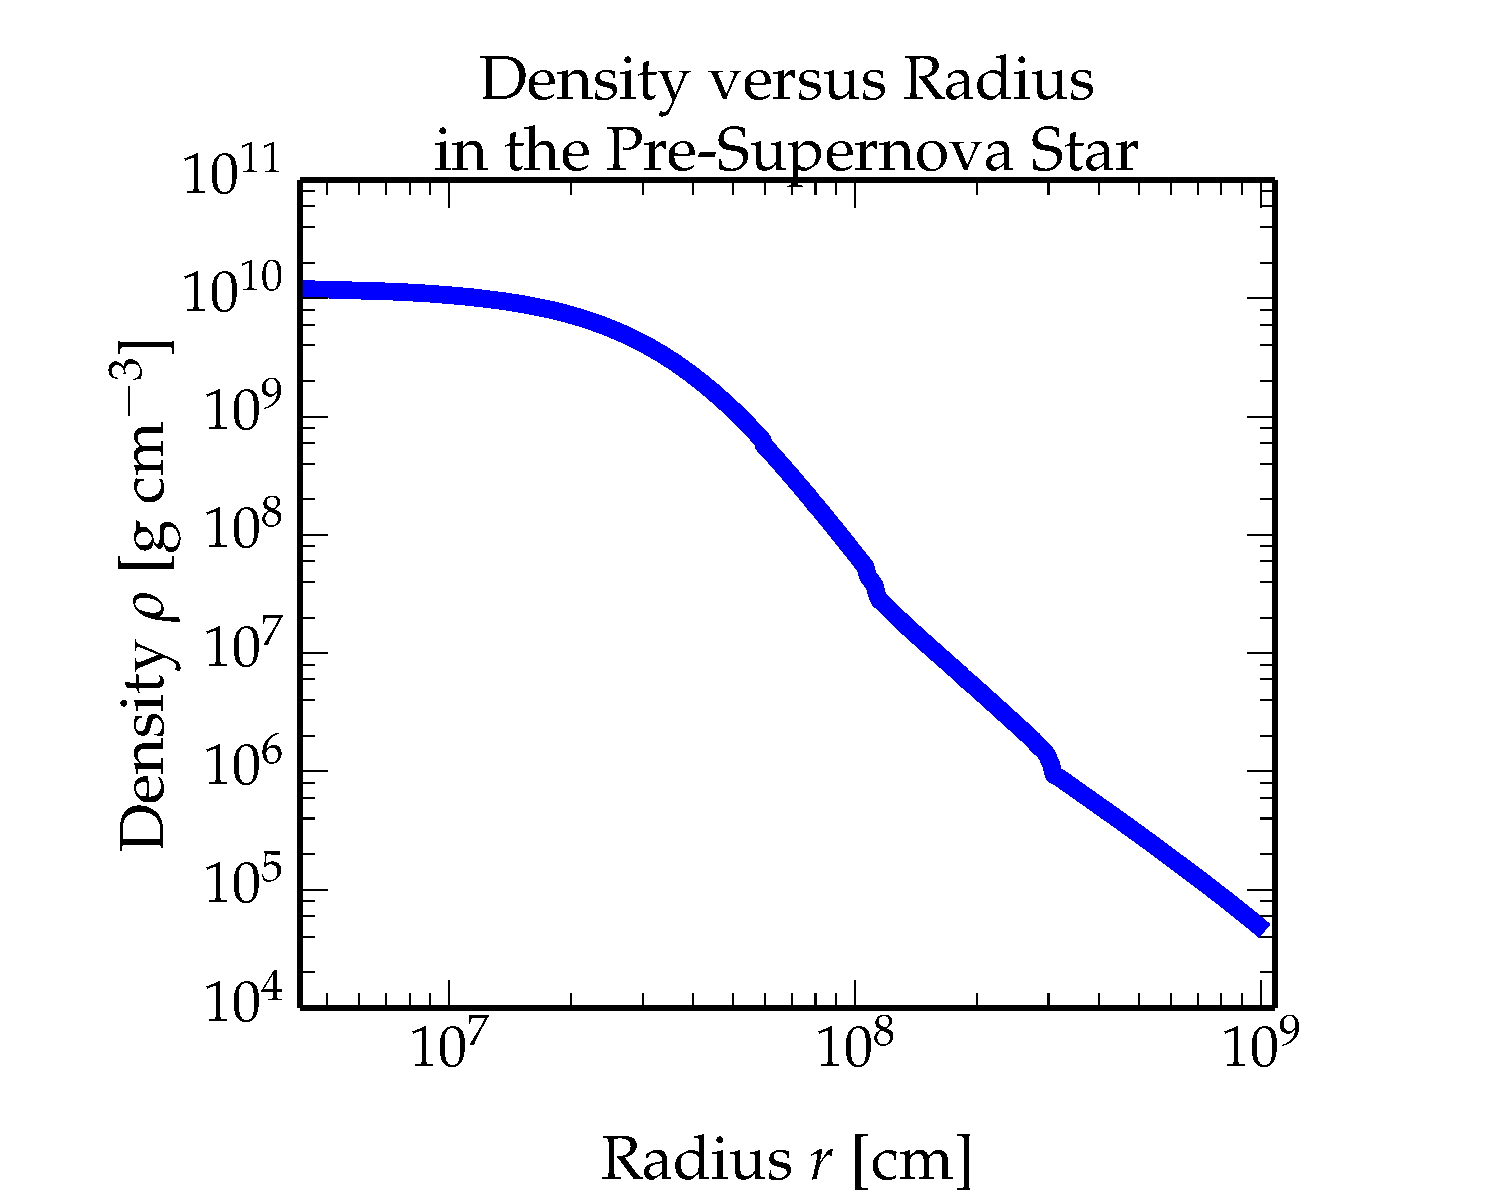
\includegraphics[width=\textwidth]{fig-density.pdf}
 \caption{Density as a function of radius in the pre-supernova star model.}
 \label{fig-density}
\end{figure} 

I then wrote an integrator for the gravitational potential \(\phi(r)\) and applied it to the case of a sphere of homogeneous density. The numerical result is compared to the analytic result in Figure~2.

\begin{figure}[H]
 \centering
 \hspace{0cm} 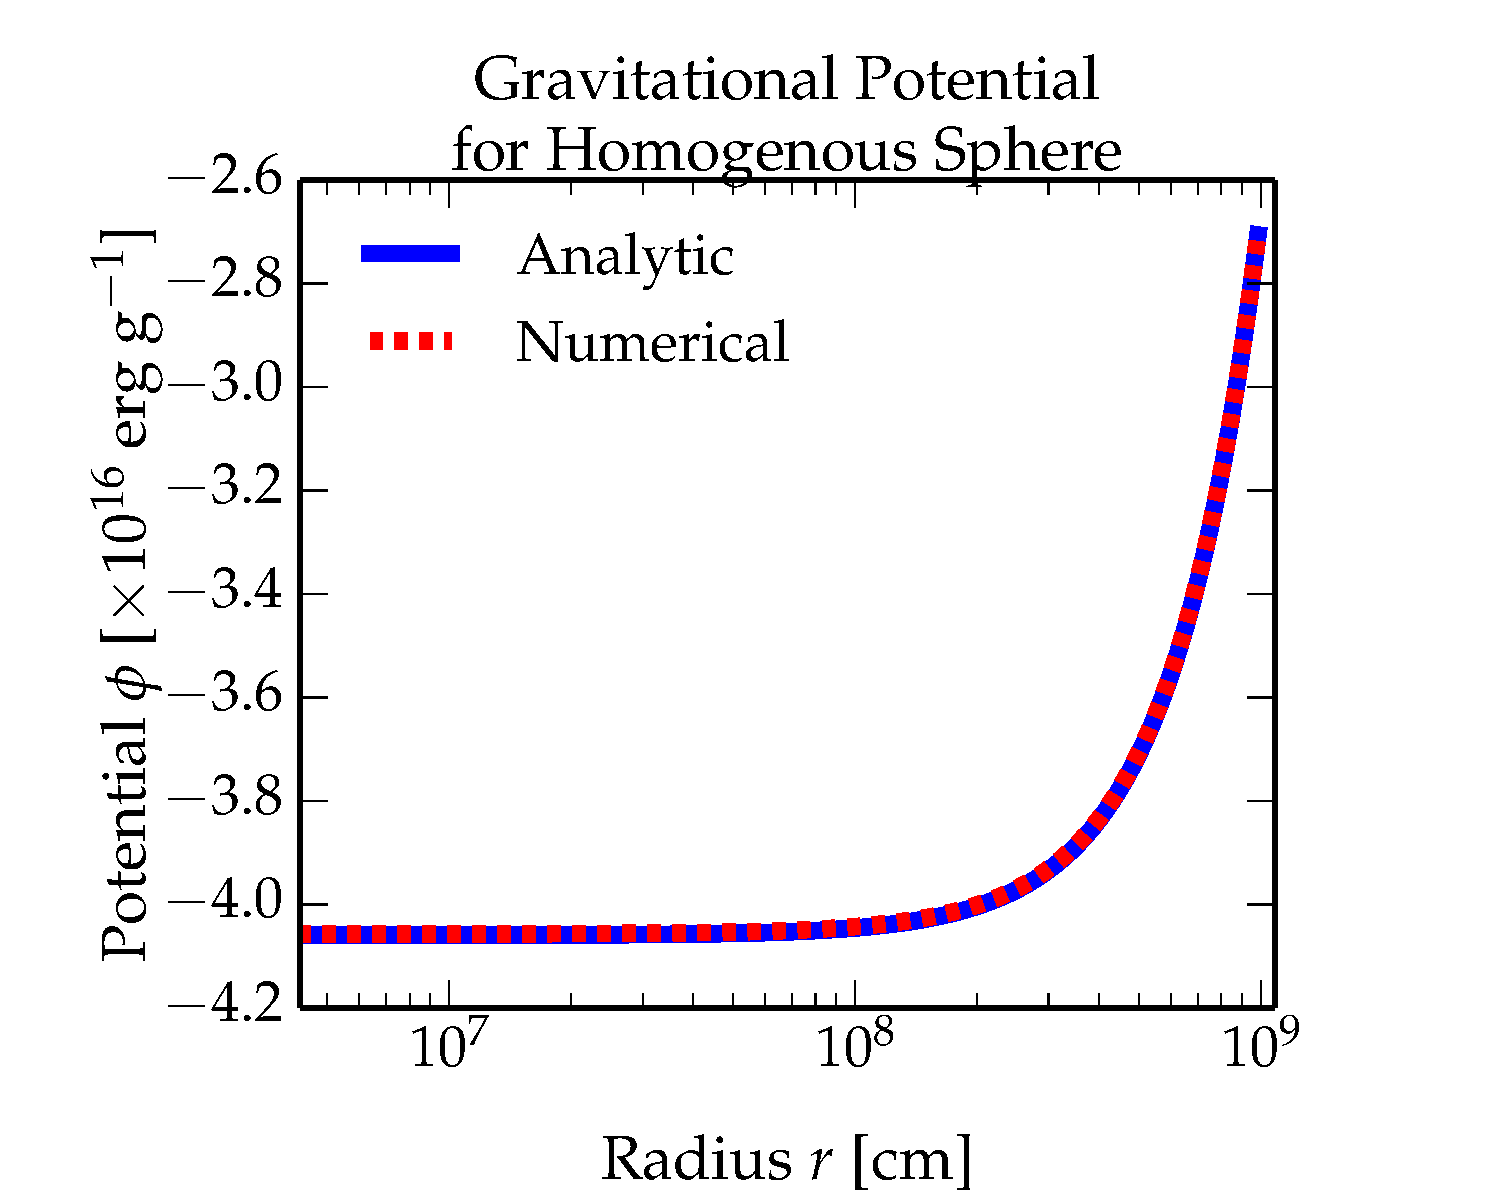
\includegraphics[width=\textwidth]{fig-potential-homogenous.pdf}
 \caption{The gravitational potential for a homogenous sphere of uniform density, \(10^5 \g\cm^{-3}\). The analytic result of \(\phi(r) = \frac{2}{3} \pi G \rho (r^2 - 3 r_\text{max}^2)\) is plotted along with the numerical solution to the spherically-symmetric Poisson equation with 2000 grid points.}
 \label{fig-potential-homogenous}
\end{figure} 

To check convergence, I calculated
\[
Q_\text{inner} \equiv \frac{\phi_{20}(r=0) - \phi(r=0)}{\phi_{40}(r=0) - \phi(r=0)} = \left( \frac{40}{20} \right)^n,
\]
\hfill where \(n\) is the convergence rate and \(\phi_N\) is the numerical solution to \(\phi\) with \(N\) grid points.

Since the Forward Euler Method, a first-order method, was used to integrate the Poisson equation, we expect the convergence rate of our algorithm to be 1, resulting in a \(Q_\text{inner}\) of 2. In fact, the measured \(Q_\text{inner}\) was 2.03869180587, close to the expected convergence rate.

\newpage

I then applied my integrator to the pre-supernova model; the potential as a function of radius is shown in Figure~3.

\begin{figure}[H]
 \centering
 \hspace{0cm} 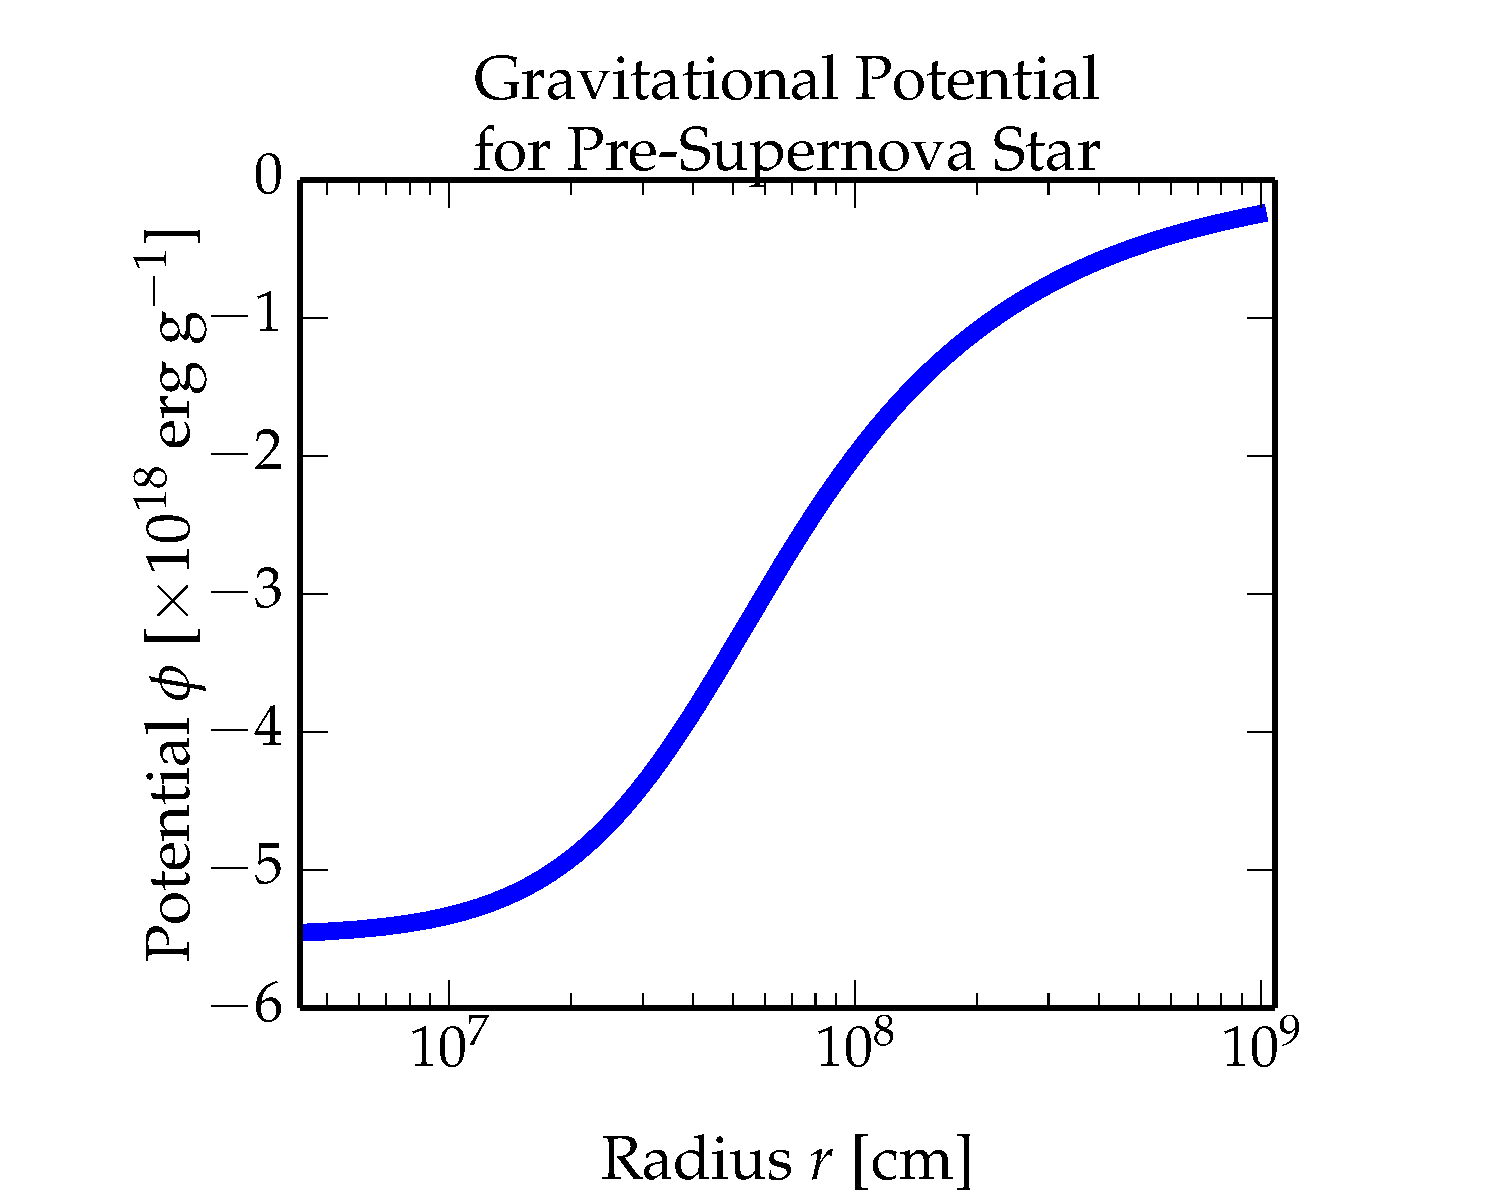
\includegraphics[width=\textwidth]{fig-potential-presupernova.pdf}
 \caption{The gravitational potential for the pre-supernova model, solved by numerical integration of the Poisson equation with 2000 grid points.}
 \label{fig-potential-presupernova}
\end{figure} 



\end{spacing}
\end{document}

%%%%%%%%%%%%%%%%%%%%%%%%%%%%%%%%%%%%%%%%%%%%%%%%%%%%%%%%%%%%%
